\documentclass[a4paper]{article}

%% Language and font encodings
\usepackage[english]{babel}
\usepackage[utf8x]{inputenc}
\usepackage[T1]{fontenc}

%% Sets page size and margins
\usepackage[a4paper,top=2cm,bottom=2cm,left=2cm,right=2cm,marginparwidth=2.75cm]{geometry}

%% Useful packages
\usepackage{amsmath}
\usepackage{graphicx}
\usepackage[colorinlistoftodos]{todonotes}
\usepackage[colorlinks=true, allcolors=blue]{hyperref}

%% Ammar Packages
\usepackage{float}
\usepackage{algpseudocode}
\usepackage{enumitem}

\title{ROB537: HW2}
\author{Ammar Kothari}
\date{}
\begin{document}
\maketitle

\section{Introduction}
Optimization through search is an important part of modern engineering.  With the advent of modern computers, people are able to generate and evaluate many solutions.  Search has been used widely in fields like engineering and finance, but has also found uses in politics \cite{totenberg_2017}.  Search is an integral part of finding solutions to challenging problems today.

In this assignment, I apply three search algorithms to solve a Travelling Salesman Problem (TSP) with 15, 25, or 100 cities that are dispersed somewhat evenly through the map.  A fourth scenario with 25 cities is structured in a way to make the solution easily identifiable.  Figure \ref{fig:15cities}, \ref{fig:25cities}, \ref{fig:100cities}, \ref{fig:25Acities} show the layout of the cities in each scenario.  The three algorithms investigated are Simulated Annealing, Genetic Algorithms, and Monte Carlo Tree Search.

\section{Problem Description}
TSP is meant to replicate the challenge of a traveller trying to visit many places without revisiting any locations.  Accordingly, the solution must contain every city only once, except for the start location.  The path must start and end at the same location.  The goal is to minimize the total cost of the path.  In this case, the cost is the distance travelled.

%!TEX root = HW2.tex
\begin{figure}[h]
	\centering
	\begin{minipage}{0.5\textwidth}
	    \centering
	    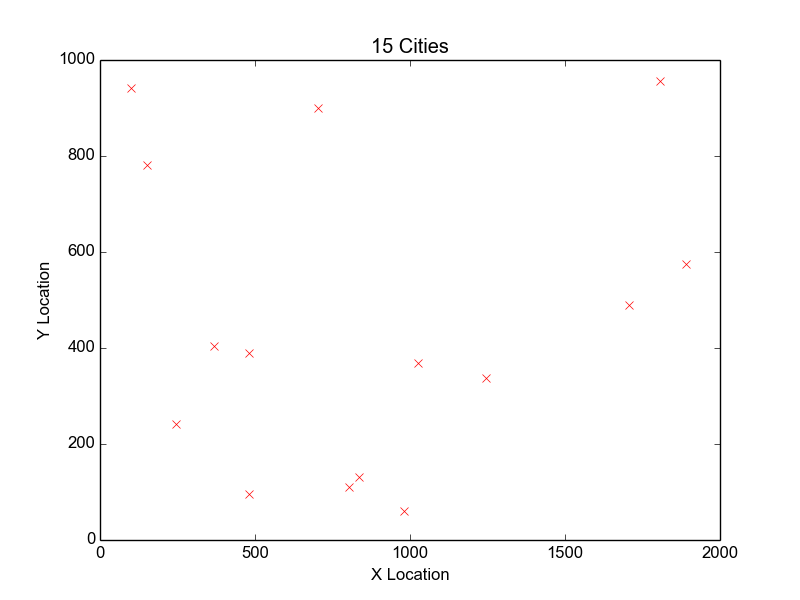
\includegraphics[width=0.9\textwidth]{15cities.png}
	    \caption{15 cities plot}
	    \label{fig:15cities}
    \end{minipage}\hfill
	\begin{minipage}{0.5\textwidth}
	    \centering
	    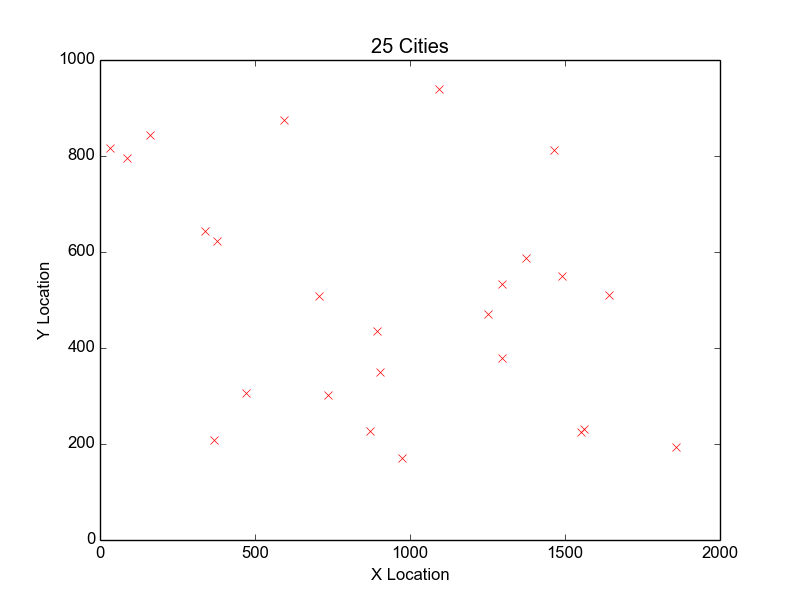
\includegraphics[width=0.9\textwidth]{25cities.png}
	    \caption{25 cities plot}
	    \label{fig:25cities}
    \end{minipage}\hfill
	\begin{minipage}{0.5\textwidth}
	    \centering
	    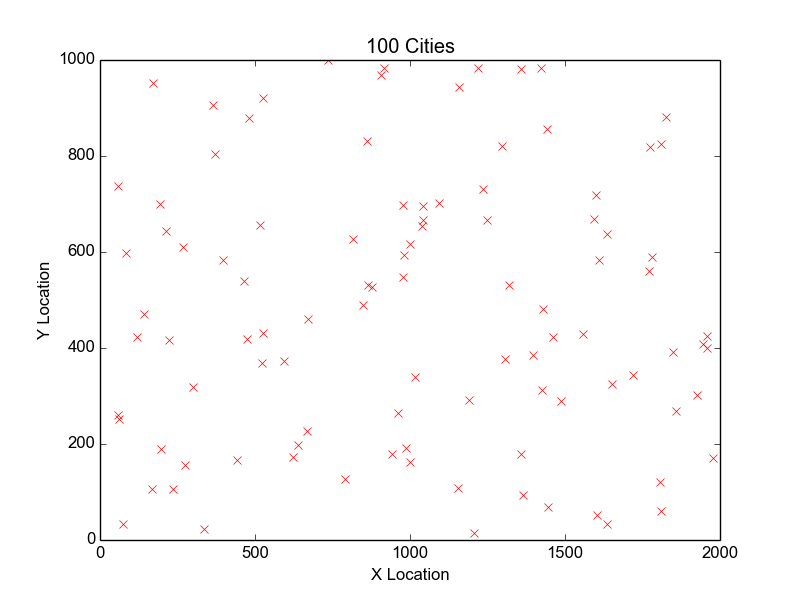
\includegraphics[width=0.9\textwidth]{100cities.png}
	    \caption{100 cities plot}
	    \label{fig:100cities}
    \end{minipage}\hfill
	\begin{minipage}{0.5\textwidth}
	    \centering
	    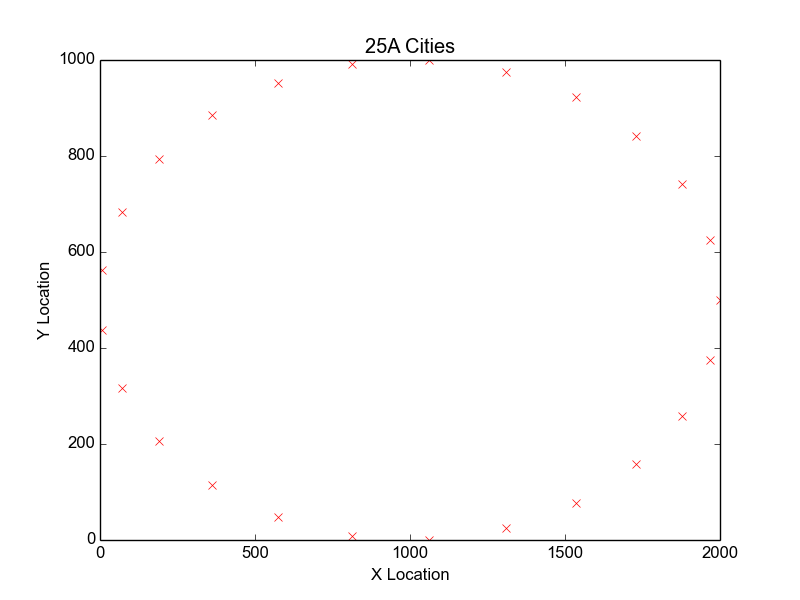
\includegraphics[width=0.9\textwidth]{25cities_A.png}
	    \caption{25 cities plot}
	    \label{fig:25Acities}
    \end{minipage}\hfill
\end{figure}

%!TEX root = HW2.tex





\section{Algorithm Explanation}
\subsection{Simulated Annealing}
% In this work, a basic version of Simulated Annealing is implementated.  
\begin{itemize}
\item s = InitialGuess()
\item For i < TOTALITERATIONS:
	\begin{itemize}
	\item sNew = NeighborSol(s)
	\item s = TempSelect(s, sNew, Temp)
	\item DecreaseTemp(Temp)
	\end{itemize}
\item FinalSolution = s
\end{itemize}

\textbf{InitialGuess} -- Intial solution generated randomly \\
\textbf{TOTALITERATIONS} -- Number of solutions to try \\
\textbf{NeighborSol} -- Generate a succesor state to $s$ by switching the order of two adjacent cities in $s$ \\
\textbf{TempSelect} -- Selects a solution between the two presented based on the temperature.  The best solution is probabilistically choosen based on the temperature.  The higher the temperature the more likely the next solution is choosen at random. \\
\textbf{DecreaseTemp} -- Decrases the temperature such that it ends at 0 (always choosing the better solution) when the maximum number of iterations is reached. 

\subsection{Evolutionary Algorithm}
% In this work, a 
\begin{itemize}
	\item POP = InitialGuess(POP\_TOT)
	\item For i < TOTALITERATIONS:
		\begin{itemize}
			\item POP\_SEL = ChooseParents(POP)
			\item CHILD = PerturbPopulation(POP\_SEL)
			\item POP = SelectPop(CHILD, POP)
		\end{itemize}
	Soltuion = Min\_Value(Pop)
\end{itemize}

\textbf{InitialGuess} -- Initial population of solutions generated randomly \\
\textbf{TOTALITERATIONS} -- Number of generations \\
\textbf{ChooseParents} -- Epsilon-greedy choose best solutions in population based on some amount of noise \\
\textbf{PerturbPopulation} -- Finds neighbor solutions based on choosen parents.  The amount of variation to original solution is based on an amount of noise.  Variation is implemented as the number of switches between neighboring cities in a solution.  Higher noise means more neighboring cities will be switched. \\
\textbf{SelectPop} -- Choose the best solutions from the original population and mutated children.  The resulting number of solutions is equal to the starting population size. \\
\textbf{Min\_Value} -- From a given population, returns the member that has the best solution value. \\

In this assignment, Population size was 10.  Number of children produced each round was 5.  Noise was decreased from 1 to 0 based on current iteration number.  For this algorithm, the total number of iterations was choosen as 1,000.  This is ten times less than the other two approaches in order to have a similar number of total generated solutions.  

\subsection{Monte Carlo Tree Search}
The implementation used in this assignment is not optimized.  As a result, it has slow run times but is able to find solutions. \\
\textbf{Main Algorithm}
\begin{itemize}
	\item InitializeTree()
	\item For i < TOTALITERATIONS:
		\begin{itemize}
			\item Parent = PickParent(Tree)
			\item Node = PickChild(Parent)
			\item Leaf\_Value = DescendTree(Node)
			\item BackPropogateValue(Leaf\_Value)
		\end{itemize}
\end{itemize}

\textbf{DescendTree}
\begin{itemize}
	\item If Node has Children
	\begin{itemize}
		\item Node = PickChild(Node)
		\item DescendTree(Node)
	\end{itemize}
	\item Else: PlayOut()
\end{itemize}

\textbf{InitializeTree} -- Initializes tree structure.  Nodes are initialized with best value to promote exploration. \\
\textbf{TOTALITERATIONS} -- Number of solutions to try \\
\textbf{PickParent} -- Probabilistically chooses the first node of the tree based on value. \\
\textbf{PickChild} -- Probabilitically choose a child from a node.  If the node does not exist, create it. \\
\textbf{DescendTree} -- Subfunction that continues to descend the tree in a probablisitic manner based on node value \\
\textbf{PlayOut} -- Determines value of a node on its first visit.  The remaining cities are choosen at random to create a valid path.  Returns the value of the full path. \\
\textbf{BackPropogateValue} -- Value of the current node is pushed to the parent.  The parent adds the new value to its current value based on the total number of visits.  For example, if a parent has been visited once before, then $(Old\_Value * Number\_Of\_Visits + New\_Child\_Value) / (Number\_Of\_Visits + 1)$.  This is effectively an average value of the node based on all explored solutions.  A node with a good value is more likely to lead to a good solution than a node with a worse value.


%!TEX root = HW2.tex
\section{15 Cities}
\subsection{Results}
For 15 cities, the algorithms all perform decently well.  The evolutionary algorithm was able to find the best solution.  SA and MCTS are both able to find near optimal algorithms.  EA takes significantly longer than the other two algorithms.  Additionally, SA has the largest variance of each iteration of all the methods between runs while EA and MCTS have similar amounts of variance in each iteration during the search process.    

One reason for EA's better performance is that it holds many more solutions in memory at a time and can compare them against each other.  The other methods hold only one or two solutions at a time and make comparisons based on those two only.  In this implementation of EA, the best solution can never be removed.  If an optimal solution is discovered, it will not be discarded which is true for MCTS, but not SA.  In all cases, EA decreases in distance the quickest.  This may be due to having acces to many solutions that it can quickly hone in on a promising solution.  Although, this may be problematic later on if this is a local minimum.

SA may struggle to get to the optimal solution if it is currently at a state that is near the optimal solution.  If more than a single switch of two consecutive states is requried to achieve a solution, then SA is unlikely to get to that solution.

MCTS has to hold a tree structure which can get quite large in memory.  Each iteration can add a new node to the tree and requires several calculations to update the tree with every iteration.  

% Put table with run time and solution quality results
\begin{table}[H]
\centering
\label{my-label}
\begin{tabular}{|c|c|c|c|c|c|}
\hline
Algorithm               & \begin{tabular}[c]{@{}c@{}}Total Solutions\\ Generated\end{tabular} & \begin{tabular}[c]{@{}c@{}}Average Min\\ Distance\end{tabular} & St Dev & \begin{tabular}[c]{@{}c@{}}Average\\ Run Time (s)\end{tabular} & St Dev \\ \hline
Simulated Annealing     & 10,000                                                              & 7,685                                                          & 994     & 4.72e-6                                                    & 3.8e-6 \\ \hline
Evolutionary Algorithm  & 10,000                                                              & 5,861                                                          & 359    & 4.39                                                       & 0.17   \\ \hline
Monte Carlo Tree Search & 10,000                                                              & 5,916                                                          & 289    & 2.19                                                       & 0.08   \\ \hline
\end{tabular}
\caption{Comparison of Solution Quality and Run Time for Each Method with 15 Cities}
\label{tab:15Comparison}
\end{table}


% insert image of example solutions found by search

\begin{figure}[H]
	\centering
    \begin{minipage}{0.45\textwidth}
        \centering
        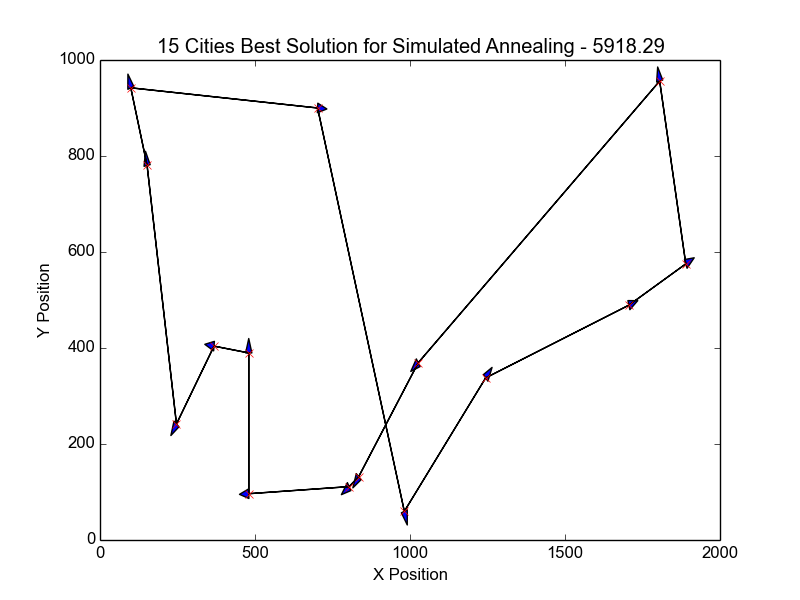
\includegraphics[width=0.9\textwidth]{15City_SA.png} % second figure itself
        \caption{Best Solution for 15 Cities with Simulated Annealing}
        \label{fig:15city_SA}
    \end{minipage}\hfill
    \begin{minipage}{0.45\textwidth}
        \centering
        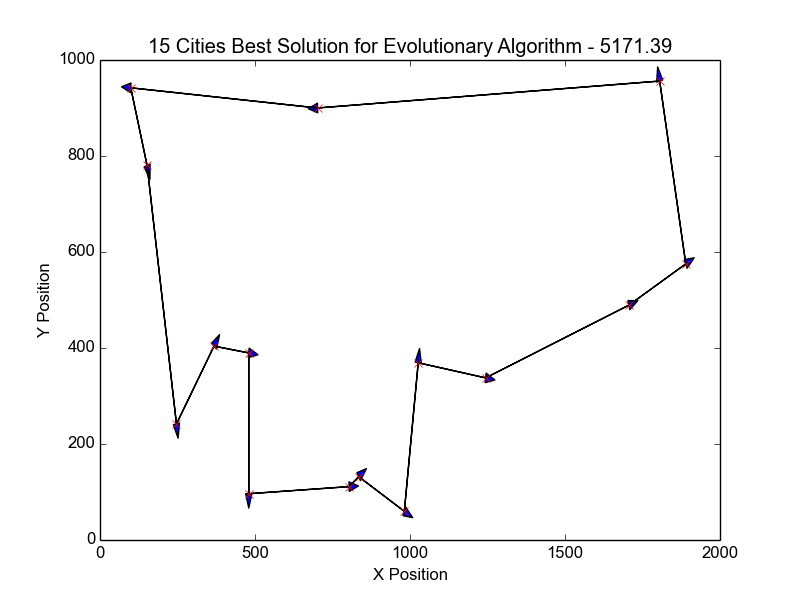
\includegraphics[width=0.9\textwidth]{15City_EA.png} % first figure itself
        \caption{Best Solution for 15 Cities with Evolutionary Algorithm}
        \label{fig:15city_EA}
    \end{minipage}\hfill
    \begin{minipage}{0.45\textwidth}
        \centering
        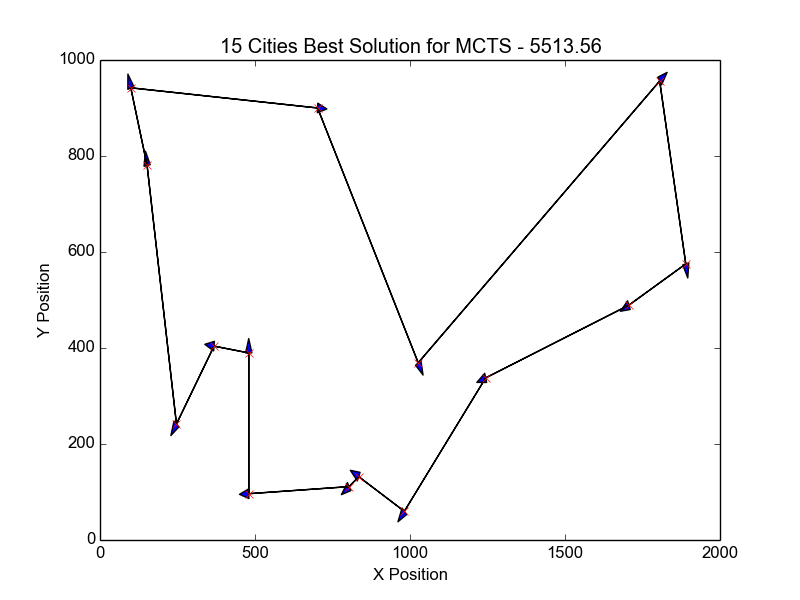
\includegraphics[width=0.9\textwidth]{15City_MCTS.png} % third figure itself
        \caption{Best Solution for 15 Cities with MCTS}
        \label{fig:15city_MCTS}
    \end{minipage}\hfill
    \begin{minipage}{0.45\textwidth}
		\centering
		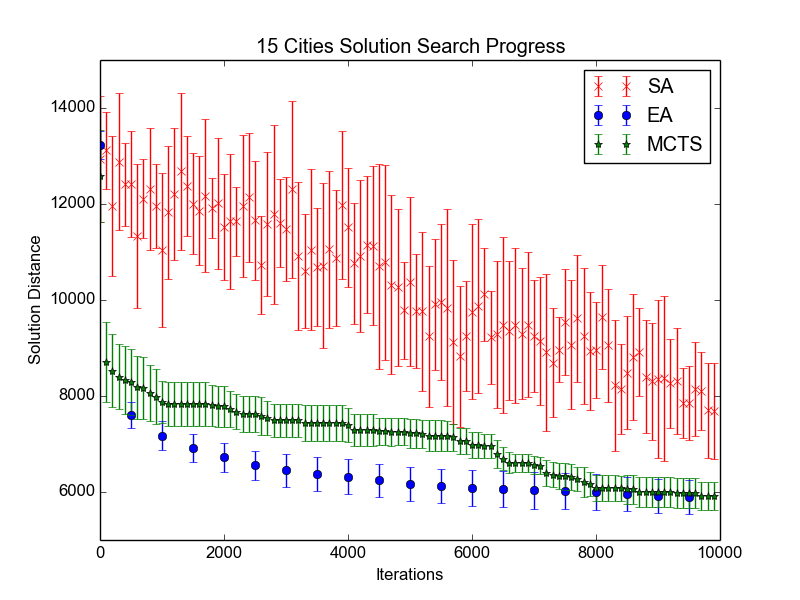
\includegraphics[width=0.9\textwidth]{15City_Solutions.png}
		\caption{Solution Progression for 15 Cities}
		\label{fig:15city_Solution}
    \end{minipage}\hfill
\end{figure}


%!TEX root = ./HW2.tex

\section{25 Cities}
\subsection{Results}
For 25 cities, the solution quality decreases.  All of the methods are not that close to the optimal solution.  EA again performs the best.  
\begin{table}[H]
\centering
\begin{tabular}{|c|c|c|c|c|c|}
\hline
Algorithm               & \begin{tabular}[c]{@{}c@{}}Total Solutions\\ Generated\end{tabular} & \begin{tabular}[c]{@{}c@{}}Average Min\\ Distance\end{tabular} & St Dev & \begin{tabular}[c]{@{}c@{}}Average\\ Run Time (s)\end{tabular} & St Dev  \\ \hline
Simulated Annealing     & 10,000                                                              & 10,598                                                         & 1,567  & 3.84e-6                                                    & 6.07e-7 \\ \hline
Evolutionary Algorithm  & 10,000                                                              & 8,035                                                          & 581    & 10.05                                                      & 0.08    \\ \hline
Monte Carlo Tree Search & 10,000                                                              & 8,693                                                          & 529    & 3.76                                                       & 0.19    \\ \hline
\end{tabular}
\caption{Comparison of Solution Quality and Run Time for Each Method with 25 Cities}
\label{tab:25Comparison}
\end{table}

% insert image of example solutions found by search

\begin{figure}[H]
	\centering
    \begin{minipage}{0.45\textwidth}
        \centering
        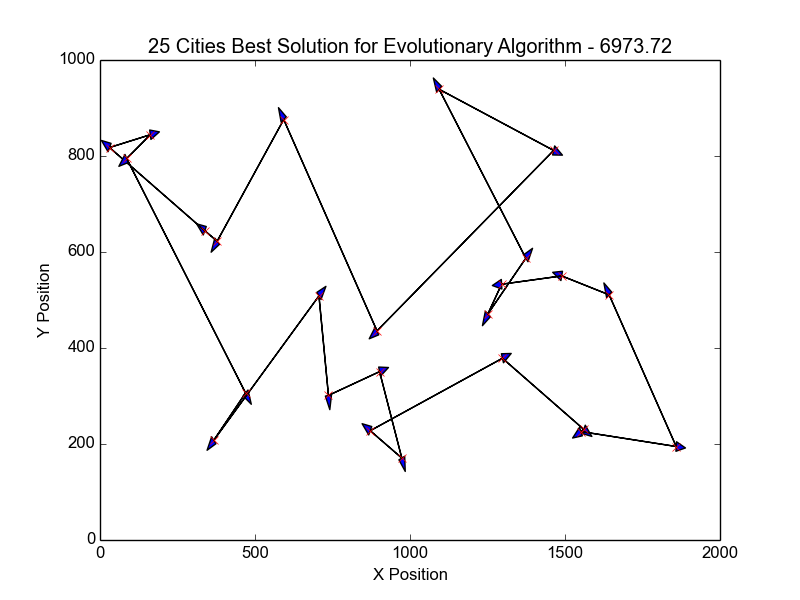
\includegraphics[width=0.9\textwidth]{25City_EA.png} % first figure itself
        \caption{Best Solution for 25 Cities with Evolutionary Algorithm}
        \label{fig:25city_EA}
    \end{minipage}\hfill
    \begin{minipage}{0.45\textwidth}
        \centering
        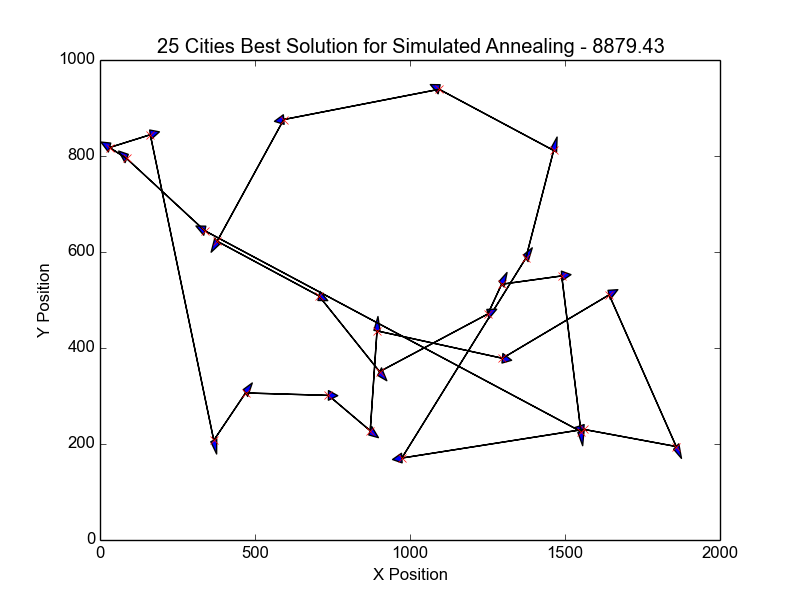
\includegraphics[width=0.9\textwidth]{25City_SA.png} % second figure itself
        \caption{Best Solution for 25 Cities with Simulated Annealing}
        \label{fig:25city_SA}
    \end{minipage}\hfill
    \begin{minipage}{0.45\textwidth}
        \centering
        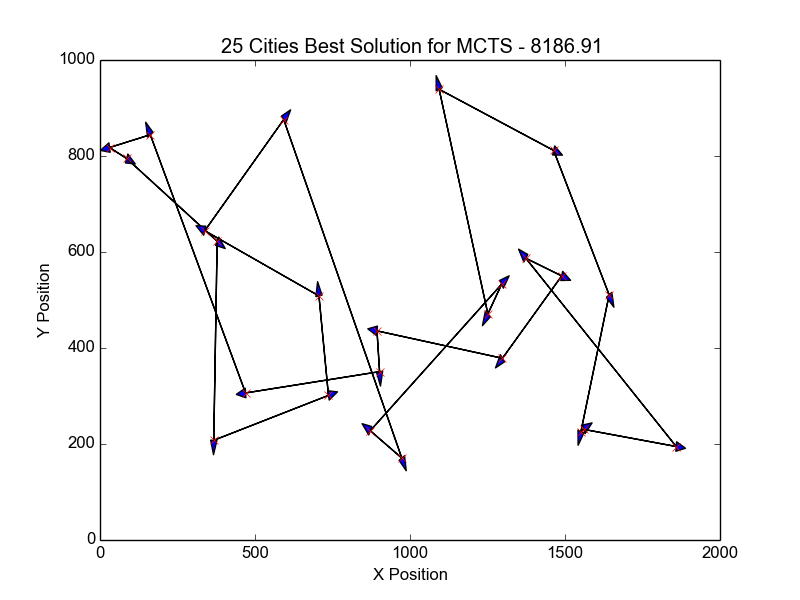
\includegraphics[width=0.9\textwidth]{25City_MCTS.png} % third figure itself
        \caption{Best Solution for 25 Cities with MCTS}
        \label{fig:25city_MCTS}
    \end{minipage}\hfill
    \begin{minipage}{0.45\textwidth}
		\centering
		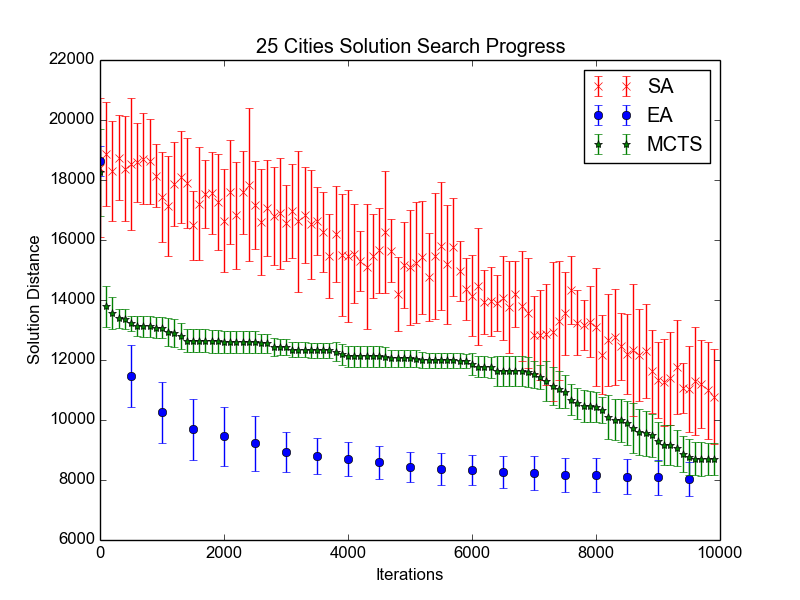
\includegraphics[width=0.9\textwidth]{25City_Solutions.png}
		\caption{Solution Progression for 25 Cities}
		\label{fig:25city_Solution}
    \end{minipage}\hfill
\end{figure}

%!TEX root = ./HW2.tex

\section{25A Cities}
\subsection{Results}
For 25 cities in a ring, EA performs best.  All of the methods struggle with overcoming paths that go vertically across the circle.  Any single switch does not lead to a better solution.  Instead, multiple swaps are required to find a better solution.  Only MCTS might be able to overcome this; looking at the solution, it seems that it is approaching a better solution, but did not have enough iterations.

The distribution of the cities affects the solution quality.  For the ring, switching two consecutive cities is all that is needed for a better solution.  This does not apply when two consecutive cities are directly across the the Y direction of the circle.  The ovalness of the distrution means directly adjacent cities are not closer.  This is a local minimum which is hard to escape.  A similar problem can be observed in the other 25 city distribution.  However, here the lack of structure in the solution makes many of the switches not as productive.  Instead, multiple consecutive city switches are required to find a better solution.  This makes the problem more challengin.  
\begin{table}[H]
\centering
\begin{tabular}{|c|c|c|c|c|c|}
\hline
Algorithm               & \begin{tabular}[c]{@{}c@{}}Total Solutions\\ Generated\end{tabular} & \begin{tabular}[c]{@{}c@{}}Average Min\\ Distance\end{tabular} & St Dev & \begin{tabular}[c]{@{}c@{}}Average\\ Run Time (s)\end{tabular} & St Dev  \\ \hline
Simulated Annealing     & 10,000                                                              & 13,796                                                         & 1,742  & 3.70e-6                                                        & 8.94e-7 \\ \hline
Evolutionary Algorithm  & 10,000                                                              & 12,222                                                         & 1,337  & 9.89                                                           & 0.03    \\ \hline
Monte Carlo Tree Search & 10,000                                                              & 12,047                                                         & 937    & 3.70                                                           & 0.15    \\ \hline
\end{tabular}
\caption{Comparison of Solution Quality and Run Time for Each Method with 25 Cities}
\label{tab:25Comparison}
\end{table}

% insert image of example solutions found by search

\begin{figure}[H]
	\centering
    \begin{minipage}{0.45\textwidth}
        \centering
        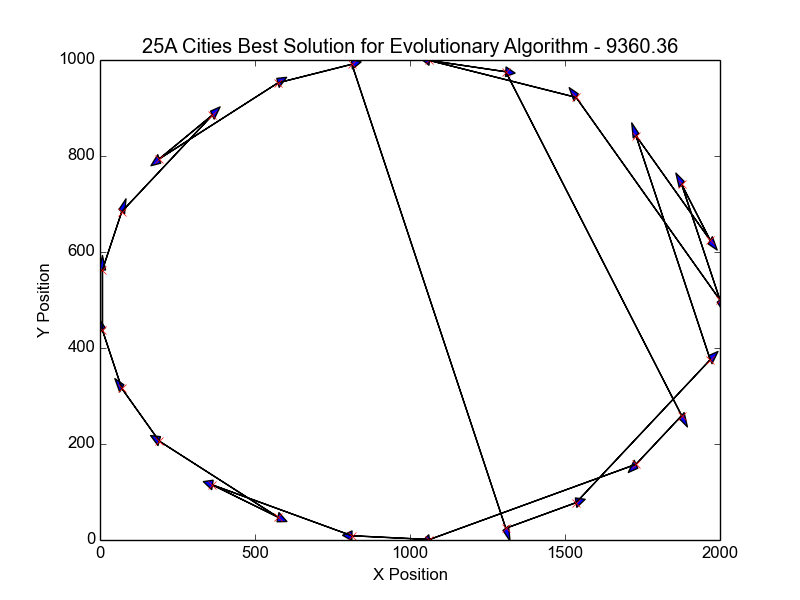
\includegraphics[width=0.9\textwidth]{25ACity_EA.png} % first figure itself
        \caption{Best Solution for 25A Cities with Evolutionary Algorithm}
        \label{fig:25Acity_EA}
    \end{minipage}\hfill
    \begin{minipage}{0.45\textwidth}
        \centering
        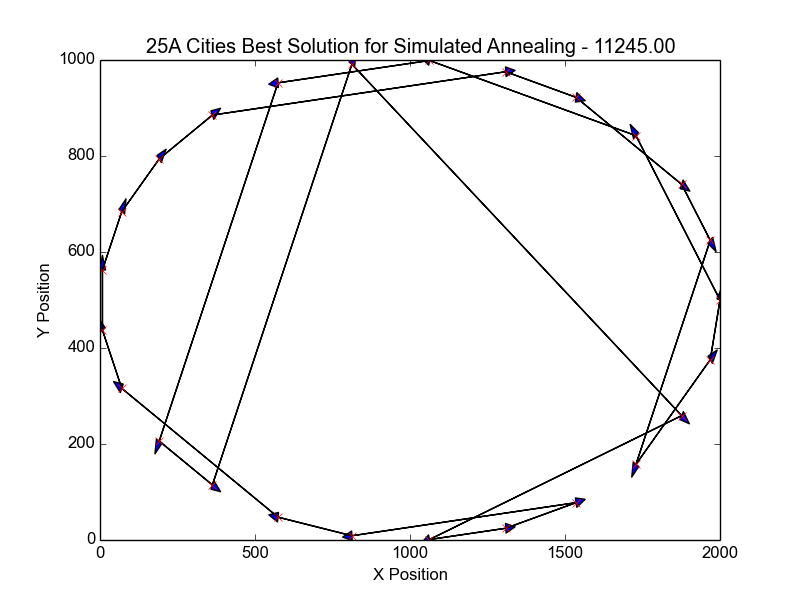
\includegraphics[width=0.9\textwidth]{25ACity_SA.png} % second figure itself
        \caption{Best Solution for 25A Cities with Simulated Annealing}
        \label{fig:25Acity_SA}
    \end{minipage}\hfill
    \begin{minipage}{0.45\textwidth}
        \centering
        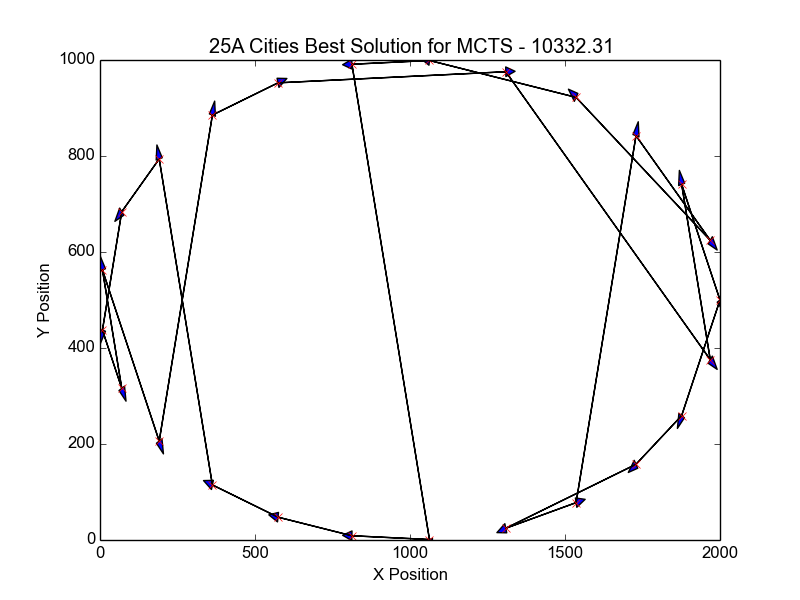
\includegraphics[width=0.9\textwidth]{25ACity_MCTS.png} % third figure itself
        \caption{Best Solution for 25A Cities with MCTS}
        \label{fig:25Acity_MCTS}
    \end{minipage}\hfill
    \begin{minipage}{0.45\textwidth}
		\centering
		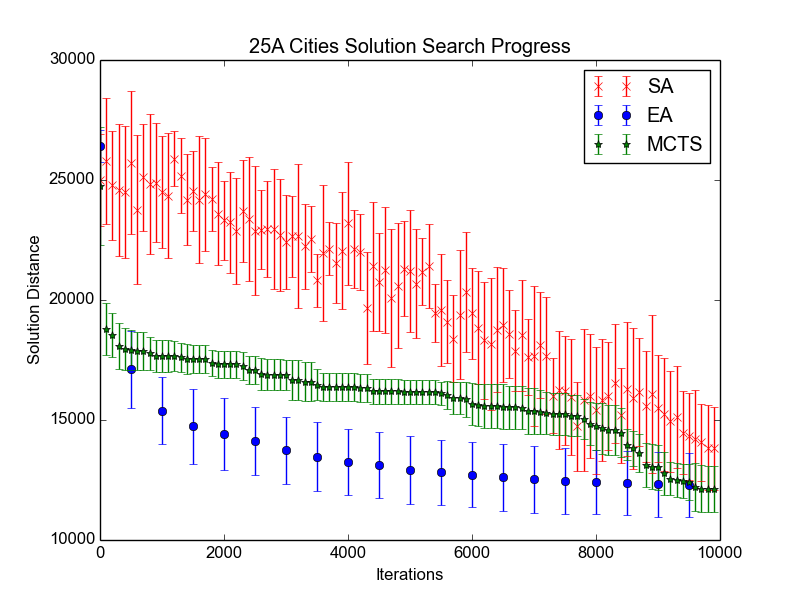
\includegraphics[width=0.9\textwidth]{25ACity_Solutions.png}
		\caption{Solution Progression for 25A Cities}
		\label{fig:25Acity_Solution}
    \end{minipage}\hfill
\end{figure}

%!TEX root = ./HW2.tex

\section{100 Cities}
\subsection{Results}
For 100 cities, the best solution is SA.  EA performs similarly, but has a larger standard deviation.  SA may be better at exploring the state space.  More variety in solution allows it to continue to hone in on a good solution.  The other two methods appear to get stuck in to a local minimum and then have trouble making large improvements from that solution.  The large exploratin also explains the steep decreasing slope for SA.


\begin{table}[H]
\centering
\begin{tabular}{|c|c|c|c|c|c|}
\hline
Algorithm               & \begin{tabular}[c]{@{}c@{}}Total Solutions\\ Generated\end{tabular} & \begin{tabular}[c]{@{}c@{}}Average Min\\ Distance\end{tabular} & St Dev & \begin{tabular}[c]{@{}c@{}}Average\\ Run Time (s)\end{tabular} & St Dev  \\ \hline
Simulated Annealing     & 10,000                                                              & 51,846                                                         & 1993  & 4.79e-6                                                        & 4.32e-7 \\ \hline
Evolutionary Algorithm  & 10,000                                                              & 57,985                                                         & 1886  & 127.00                                                           & 0.47    \\ \hline
Monte Carlo Tree Search & 10,000                                                              & 63,638                                                         & 1865    & 18.70                                                           & 0.59    \\ \hline
\end{tabular}
\caption{Comparison of Solution Quality and Run Time for Each Method with 100 Cities}
\label{tab:100Comparison}
\end{table}

% insert image of example solutions found by search

\begin{figure}[H]
	\centering
    \begin{minipage}{0.45\textwidth}
        \centering
        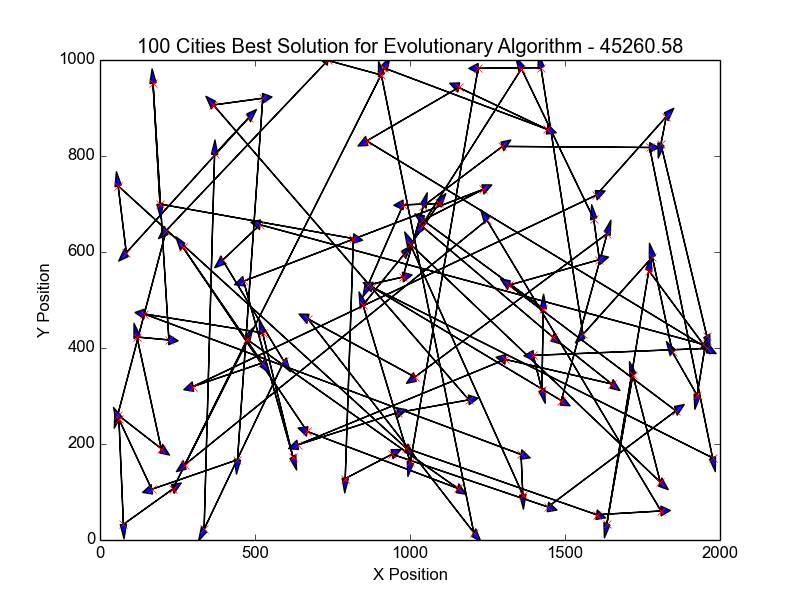
\includegraphics[width=0.9\textwidth]{100City_EA.png} % first figure itself
        \caption{Best Solution for 100 Cities with Evolutionary Algorithm}
        \label{fig:100city_EA}
    \end{minipage}\hfill
    \begin{minipage}{0.45\textwidth}
        \centering
        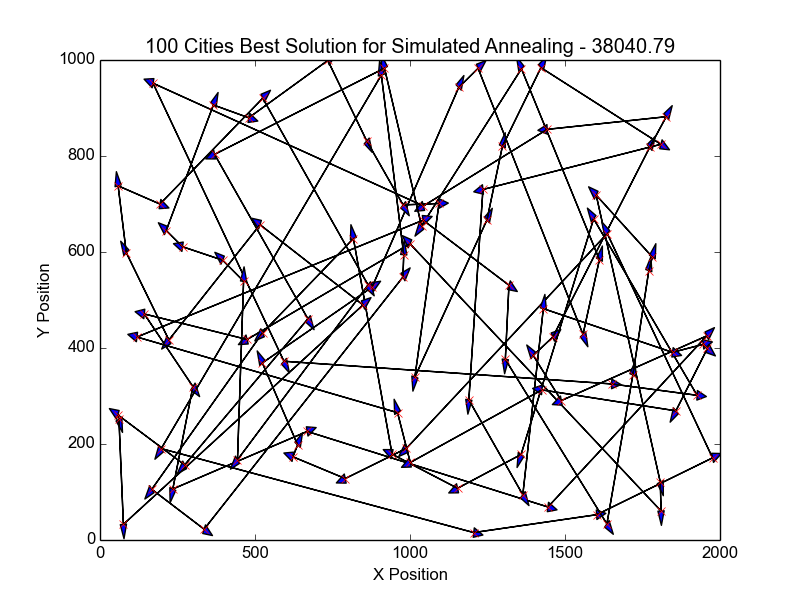
\includegraphics[width=0.9\textwidth]{100City_SA.png} % second figure itself
        \caption{Best Solution for 100 Cities with Simulated Annealing}
        \label{fig:100city_SA}
    \end{minipage}\hfill
    \begin{minipage}{0.45\textwidth}
        \centering
        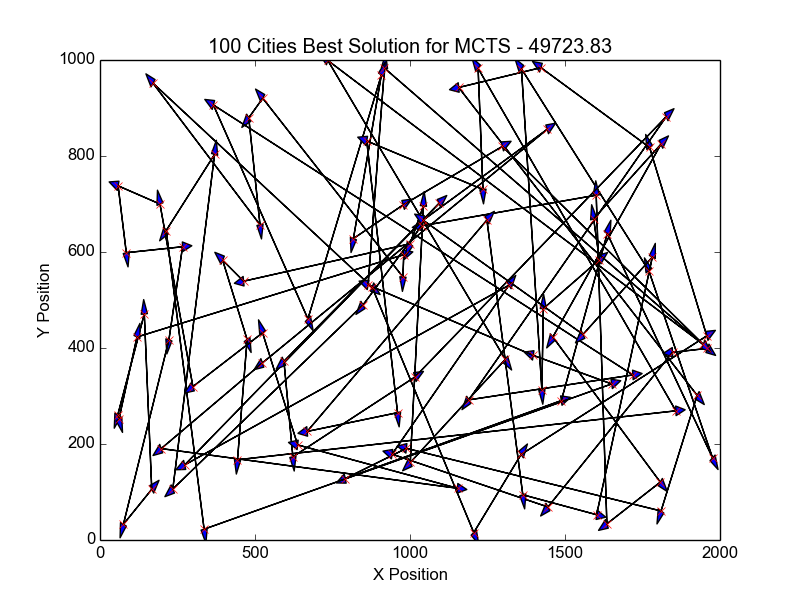
\includegraphics[width=0.9\textwidth]{100City_MCTS.png} % third figure itself
        \caption{Best Solution for 100 Cities with MCTS}
        \label{fig:100city_MCTS}
    \end{minipage}\hfill
    \begin{minipage}{0.45\textwidth}
		\centering
		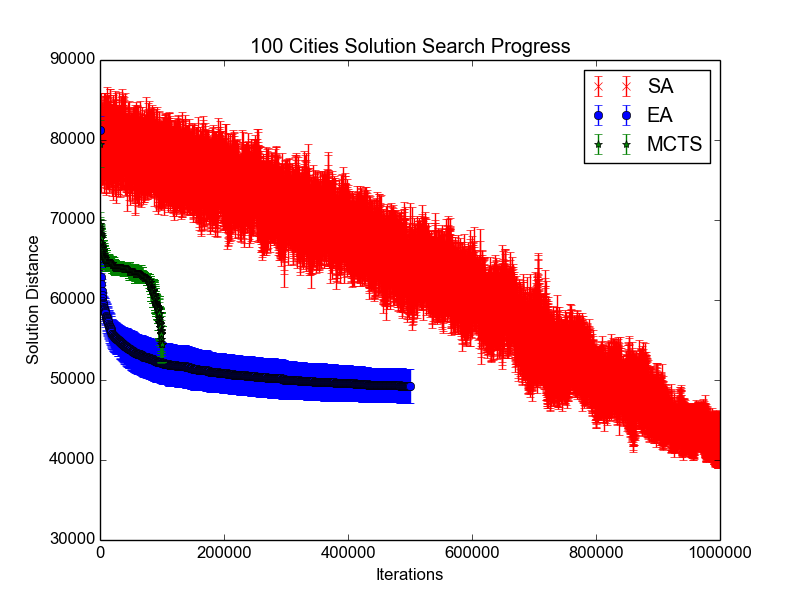
\includegraphics[width=0.9\textwidth]{100City_Solutions.png}
		\caption{Solution Progression for 100 Cities}
		\label{fig:100city_Solution}
    \end{minipage}\hfill
\end{figure}



%!TEX root = ./HW2.tex


\section{Solution Size}
As the number of cities to traverse increases, the possible solutions increases which makes search harder.  For all the experiments run in this assignment, 10,000 solutions were generated before stopping the search.  A generated solution could have been a duplicate of a solution already produced.  As a result, the number of solutions searched over cannot be determined for sure.  However, as an upper bound, the uniquenes of solutions will be assumed.  

\bibliographystyle{unsrt}
\bibliography{HW2}

\end{document}	